\documentclass[a4paper,landscape]{article}
\usepackage[pdftex,hidelinks]{hyperref}
\usepackage{fancyhdr}
\usepackage[
  headheight=35pt,
  headsep=15pt,
  footskip=20pt,
  includeheadfoot,
  hmargin=1cm,
  vmargin=0.75cm
]{geometry}
\usepackage{multirow}
\usepackage{tabularx}
\usepackage{tikz}

\pagestyle{fancy}
\tikzset{baseline=0,>=stealth}
\setlength{\parindent}{0pt}
\setlength{\tabcolsep}{10pt}
\renewcommand{\arraystretch}{1.5}

\title{Flatwater Kayaking}
\author{Jouke~Witteveen}

\makeatletter
\hypersetup{pdftitle=\@title,pdfauthor=\@author,pdfsubject={Technical Template: Style}}
\lhead{}
\chead{
  \LARGE{\textbf{\@title}} \\[4pt]
  \large{Technical Template --- Style}
}
\rhead{}
\lfoot{}
\cfoot{}
\rfoot{\small{\copyright{}~\the\year{} \@author}}
\makeatother


\begin{document}

\hspace{0pt}\vspace{\stretch{1}} \\[-\baselineskip]
\begin{tabularx}{\textwidth}{cp{9.7em}*{3}{|X}}
\multicolumn{2}{c}{}	& \multicolumn{3}{c}{
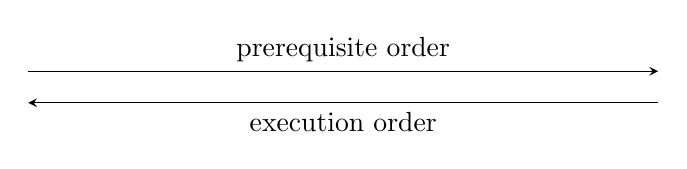
\begin{tikzpicture}
  \draw[->] (-4, 0.2) -- (4, 0.2) node[midway,above] {prerequisite order};
  \draw[<-] (-4, -0.2) -- (4, -0.2) node[midway,below] {execution order};
\end{tikzpicture}} \\[20pt]
\multicolumn{2}{c|}{}	& \multicolumn{1}{c|}{\emph{\textbf{Pull}}}	& \multicolumn{1}{c|}{\emph{\textbf{Entry}}}	& \multicolumn{1}{c}{\emph{\textbf{Set-up / Exit}}} \\
\cline{2-5}
\multirow{16.3}{*}{ % nrows = 3 + (lines - 3) / \arraystretch
\hspace{-20pt}
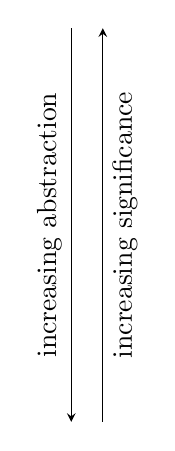
\begin{tikzpicture}
  \draw[<-] (-0.2, -2.5) -- (-0.2, 2.5) node[midway,sloped,above] {increasing abstraction};
  \draw[->] (0.2, -2.5) -- (0.2, 2.5) node[midway,sloped,below] {increasing significance};
\end{tikzpicture}
\hspace{0pt}}
& \emph{All applied forces must contribute to desirable acceleration.}
	& There should be no forward movement relative to the boat of the side of the hip furthest away from the submersed blade.
	  All action of the leg closest to the submersed blade should directly result in acceleration of the boat.
	  Forces on the back of the seat and on the pull bar should be minimized.
	& The blade should enter the water at maximum reach, when the top arm is bent, the torso rotated, and the pulling arm extended.
	  The top arm transfers a vertical force between the body and the paddle shaft, and should not yield forward or upward during the entry of the blade.
	& The top hand should only move forward after the pressure is removed from the submersed blade and it should not move down before the blade is completely out of the water.
	  This establishes a high fulcrum for the paddle as a lever.
	  The extraction of the blade should be swift and smooth. \\
\cline{2-5}
& \emph{Hydrodynamic properties of the paddle blade and the hull of the boat must be utilized to maximize the yield from every stroke.}
	& The submersed blade should not move backward relative to the water.
	  The blade should be pushed away from the boat using the sideward resistance of the hull of the boat in the water.
	  The top hand and the bottom hand should move sideward in tandem.
	& Weight should be shifted slightly toward the side of the boat where the blade is about to enter the water.
	  Entry of the blade into the water should be forceful and with an emphasis on a high downward directed velocity.
	  The forward directed lift force should immediately be transferred to the boat via the pulling arm.
	& The extraction of the blade from the water should start shortly after the blade moves past its vertical position in the water.
	  Paddle spray should be minimized.
	  At the water surface, spray should be directed away from the boat and possibly backward, but never forward.
	  Weight should be kept close to the centerline of the boat. \\
\cline{2-5}
& \emph{Acceleration of the center of mass must be decoupled from the velocity of the boat.}
	& Body rotation should happen on the axis running through the side of the hip furthest away from the submersed blade and the shoulder closest to the submersed blade.
	  The center of the chest should move forward relative to the boat without moving downward.
	  The boat should move through the water smoothly.
	& An upright posture, without forward lean, should be assumed during the acceleration of the blade toward the water.
	  Seen from behind, the spine should not bend to either side.
	  The downward directed acceleration of the blade should not result in noticeable upward movement of the boat.
	& After the pressure is removed from the blade, the upper body should start moving backward relative to the boat.
	  The smooth movement of the boat through the water should be continued via pressure on the front of the seat without putting pressure on the pull bar.
\end{tabularx}
\vspace{\stretch{2}}

\small{
\emph{Pressure} is defined as force per unit area.
For a fixed area, the pressure is proportional to the force and we may use both terms interchangeably in a qualitative analysis.
}

\end{document}
